\section{三角形网格}\label{sec:三角形网格}
\keyindex{三角形}{triangle}{}是计算机图形学最常用的形状;
复杂场景会用上百万三角形建模以实现出色细节
(\reffig{3.11}展示了四百多万三角形的复杂三角网格图像)。
\begin{figure}[htbp]
    \centering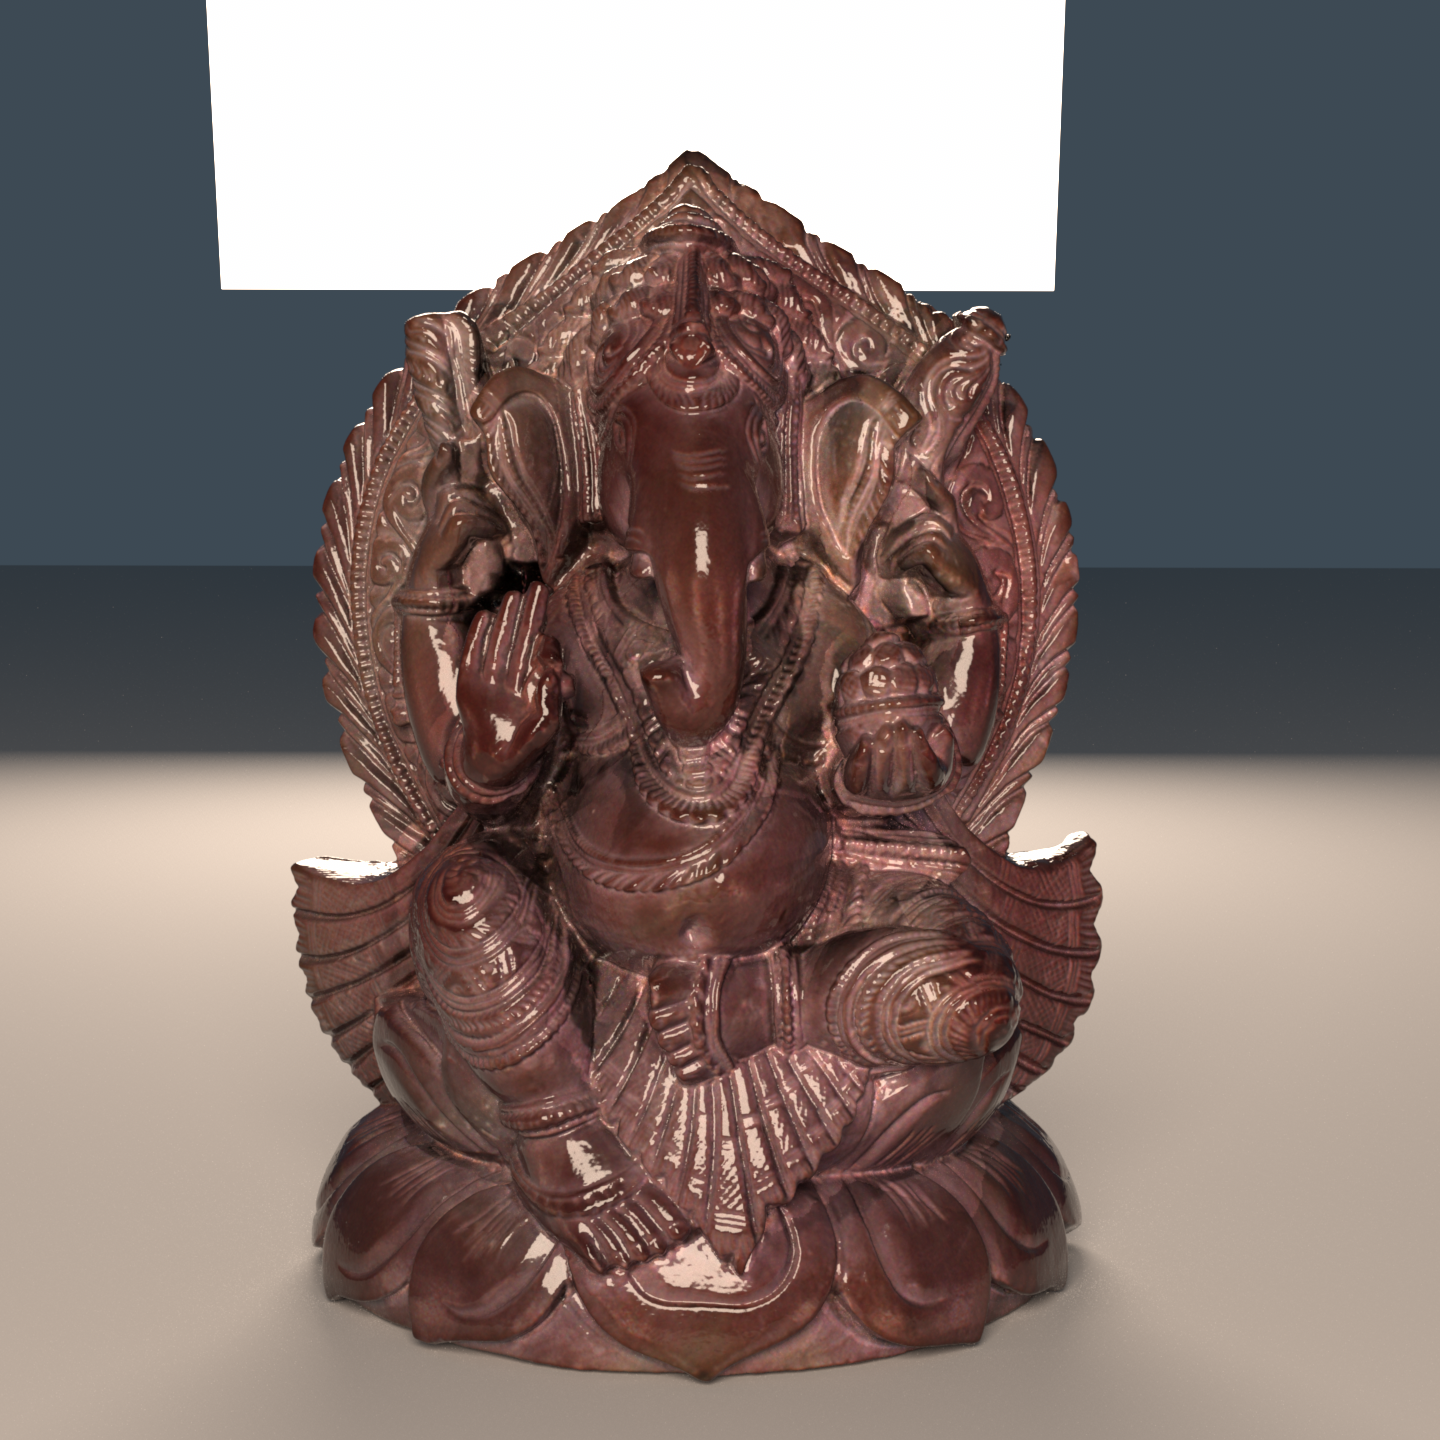
\includegraphics[width=\linewidth]{chap03/ganesha.png}
    \caption{象头神模型。该三角网格含有四百多万个独立三角形。
        它是使用结构光确定物体形状的3D扫描器用真实雕塑创建的。}
    \label{fig:3.11}
\end{figure}

尽管自然的表示是用{\ttfamily Triangle}形状实现,
每个三角形都存储它三个顶点的位置,
但内存更高效的表示是用一个顶点位置数组分开存储整个三角网格,
每个独立三角形只存储它三个顶点对该数组的三个偏移量。

为了理解为什么是这样,考虑著名的\keyindex{欧拉-庞加莱公式}{Euler-Poincaré formula}{},
它将闭合离散网格的顶点数$V$、边数$E$和面数$F$联系起来:
\begin{align*}
    V-E+F=2(1-g)\, ,
\end{align*}
其中$g\in\mathbb{N}$是网格的\keyindex{亏格}{genus}{}。
亏格通常是很小的数且能解释为网格的“手柄”数量(类似于茶杯把手)。
在三角网格上,边数和面数\sidenote{译者注:原文错写为顶点数,已修改。}还由恒等式联系
\begin{align*}
    E=\frac{3}{2}F\, .
\end{align*}
这可以看作把每条边分成两部分与两个相邻三角形关联。
有$3F$条这样的半边,所有同位的边对构成$E$条网格边。
对于巨大的闭合三角网格,亏格的整体影响通常可以忽略,
我们可以结合之前两个方程(以及$g=0$)得到
\begin{align*}
    F\approx2V\, .
\end{align*}
换句话说,面数大约是顶点数的两倍。
既然每个面引用三个顶点,每个顶点(平均)总共被引用六次。
因此当共享顶点时,每个三角形所需的总分摊存储为
偏移量的12字节内存(三个4字节32位整数偏移量)加上一个顶点存储的一半——6字节,
这里假设每个顶点用三个4字节浮点存储——每个三角形一共18字节。
这比每个三角形直接用36字节存储三个位置好得多。
当网格中有每个顶点的曲面法线或纹理坐标时,相对的存储节约会更好。

pbrt使用结构体\refvar{TriangleMesh}{}保存关于三角网格的共享信息。
\begin{lstlisting}
`\initcode{Triangle Declarations}{=}\initnext{TriangleDeclarations}`
struct `\initvar{TriangleMesh}{}` {
    `\refcode{TriangleMesh Public Methods}{}`
    `\refcode{TriangleMesh Data}{}`
};
\end{lstlisting}
\begin{lstlisting}
`\initcode{TriangleMesh Public Methods}{=}`
`\refvar{TriangleMesh}{}`(const `\refvar{Transform}{}` &ObjectToWorld, int nTriangles, const int *vertexIndices,
    int nVertices, const `\refvar{Point3f}{}` *P, const `\refvar{Vector3f}{}` *S, const `\refvar{Normal3f}{}` *N,
    const `\refvar{Point2f}{}` *uv, const std::shared_ptr<`\refvar{Texture}{}`<`\refvar{Float}{}`>> &alphaMask);
\end{lstlisting}

\refvar{TriangleMesh}{}构造函数的参数如下:
\begin{itemize}
    \item {\ttfamily ObjectToWorld}:网格的物体到世界的变换。
    \item {\ttfamily nTriangles}:网格中三角形总数。
    \item {\ttfamily vertexIndices}:指向顶点索引数组的指针。对于第{\ttfamily i}个三角形,其三个顶点位置为
          {\ttfamily P[vertexIndices[3*i]]}、{\ttfamily P[vertexIndices[3*i+1]]}和{\ttfamily P[vertexIndices[3*i+2]]}。
    \item {\ttfamily nVertices}:网格中顶点总数。
    \item {\ttfamily P}:{\ttfamily nVertices}个顶点位置的数组。
    \item {\ttfamily S}:可选切向量数组,网格中每个顶点都有一个。它们用于计算着色切线。
    \item {\ttfamily N}:可选法向量数组,网格中每个顶点都有一个。如果有,则它们在三角形面之间插值以计算着色法线。
    \item {\ttfamily UV}:可选参数值$(u,v)$数组,每个顶点一个。
    \item {\ttfamily alphaMask}:可选的\keyindex{$\alpha$掩模}{alpha mask}{}纹理,可用于截去部分三角形面。
\end{itemize}